%!TEX TS-program = xelatex
%!TEX encoding = UTF-8 Unicode

\documentclass[12pt]{extarticle}
% extarticle is like article but can handle 8pt, 9pt, 10pt, 11pt, 12pt, 14pt, 17pt, and 20pt text

\def \ititle {Origins of Mind}
 
\def \isubtitle {Lecture 08}
 
\def \iauthor {Stephen A. Butterfill}
\def \iemail{s.butterfill@warwick.ac.uk}
\date{}

%for strikethrough
\usepackage[normalem]{ulem}

\input{$HOME/Documents/submissions/preamble_steve_handout}

%\bibpunct{}{}{,}{s}{}{,}  %use superscript TICS style bib
%remove hanging indent for TICS style bib
%TODO doesnt work
\setlength{\bibhang}{0em}
%\setlength{\bibsep}{0.5em}


%itemize bullet should be dash
\renewcommand{\labelitemi}{$-$}

\begin{document}

%\raggedcolumns

\begin{multicols*}{3}

\setlength\footnotesep{1em}


\bibliographystyle{newapa} %apalike

%\maketitle
%\tableofcontents




%--------------- 
%--- start paste

\def \ititle {Logic I}
 
\def \isubtitle {Fast Lecture 01}
 
\begin{center}
 
{\Large
 
\textbf{\ititle}: \isubtitle
 
}
 
 
 
\iemail %
 
\end{center}
 
Readings refer to sections of the course textbook, \emph{Language, Proof and Logic}.
 
 
 
\section{Terminology}
 
\begin{center}
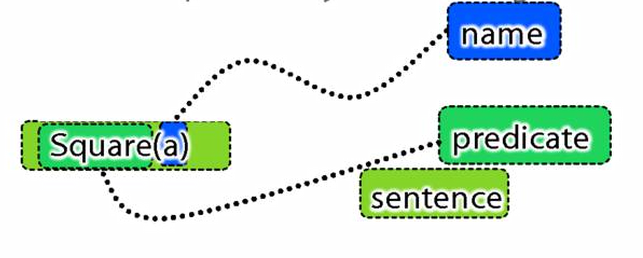
\includegraphics[scale=0.3]{img/name_predicate_sentence.png}
\end{center}
 
 
\section{Logically Valid Arguments}
 
\emph{Reading:} §2.1
 
An argument is \emph{logically valid} just if there’s no possible situation in which the premises are true and the conclusion false
 
A \emph{connective} joins one or more sentences to make a new sentence. E.g. ‘because’, ‘¬’. The sentences joined by a connective are called \emph{constituent sentences}.
 
E.g. in ‘P $\lor{}$ Q’,
 
\begin{quote}
 
$\lor{}$ is the connective
 
P, Q are the constituent sentences
 
\end{quote}
 
\begin{center}
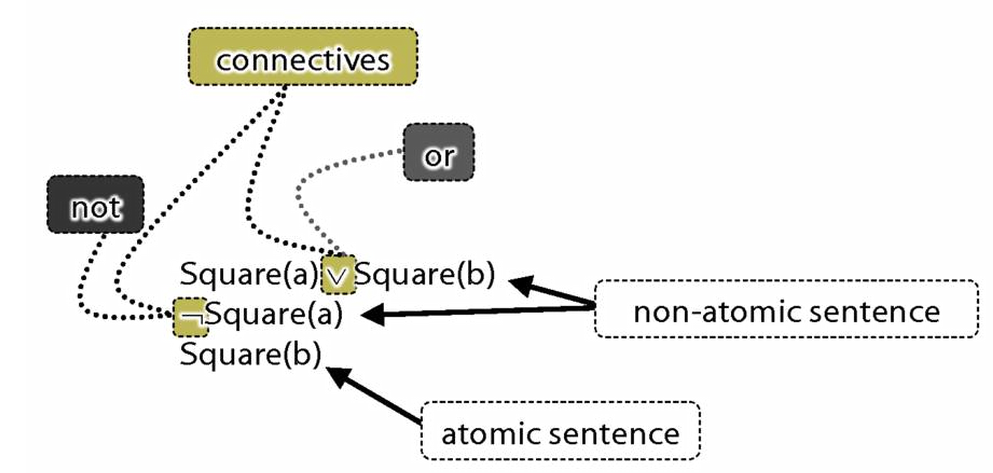
\includegraphics[scale=0.3]{img/terminology_more.png}
\end{center}
 
 
\section{Sentence Letters}
 
\begin{center}
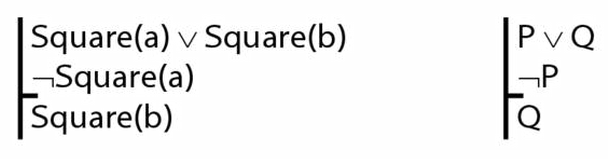
\includegraphics[scale=0.3]{img/sentence_letters.png}
\end{center}
 
 
\section{Counterexamples}
 
\emph{Reading:} §2.5
 
A \emph{counterexample} to an argument is a possible situation in which its premises are T and its conclusion F.
 
There are no counterexamples to a logically valid argument.
 
If an argument is not valid, then there is a counterexample to it.
 
To show that an argument is not logically valid, we specify a counterexample to it.
 
 
 
\section{Identity}
 
\emph{Reading:} §2.2
 
Principle: If b=c then whatever is true of b is also true of c.
 
Principle: a=a is never false
 
\begin{center}
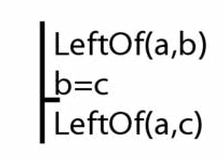
\includegraphics[scale=0.3]{img/arg_identity.png}
\end{center}
 
 
\section{Truth Tables}
 
\emph{Reading:} §3.1, §3.2, §3.3
 
Rough guide:
 
`$\land{}$' means and
 
`$\lor{}$' means or
 
`$\lnot{}$' means not
 
\begin{center}
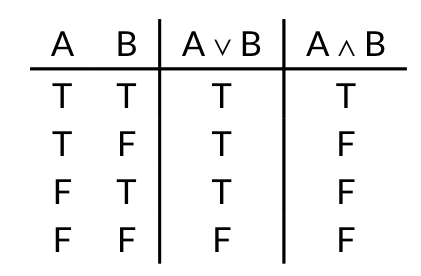
\includegraphics[scale=0.3]{img/truth_table_or_and.png}
\end{center}
\begin{center}
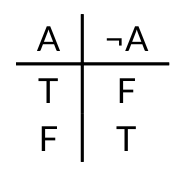
\includegraphics[scale=0.3]{img/truth_table_not.png}
\end{center}
 
 
\section{Complex Truth Tables}
 
\emph{Reading:} §3.3, §3.5
 
\begin{center}
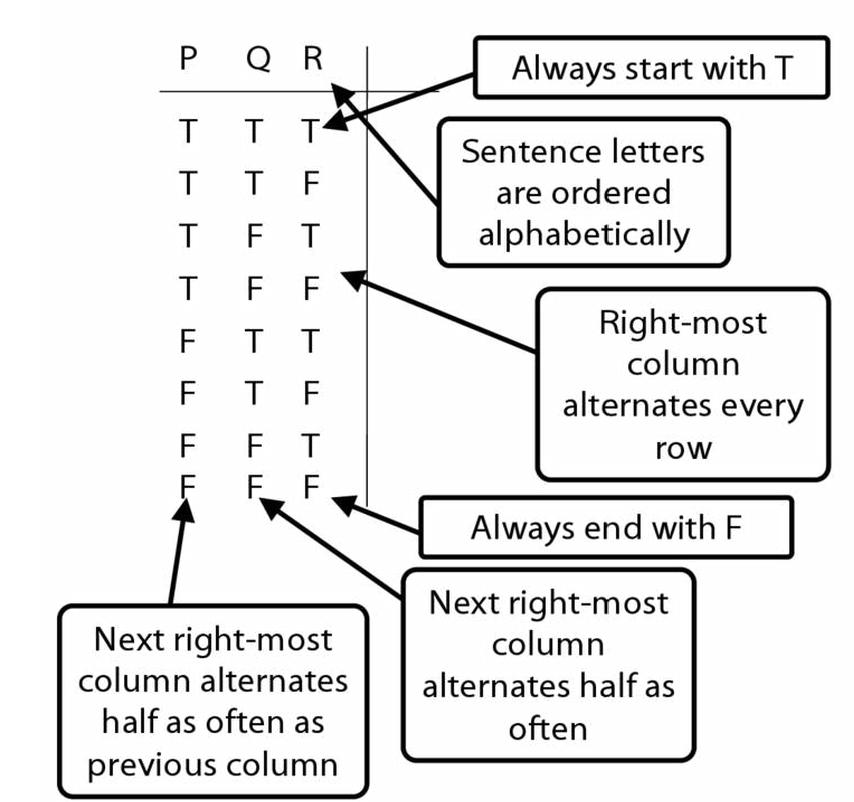
\includegraphics[scale=0.3]{img/how_to_write_truth_tables.png}
\end{center}
\begin{minipage}{\columnwidth}
 
Complex truth table example:
 
\begin{center}
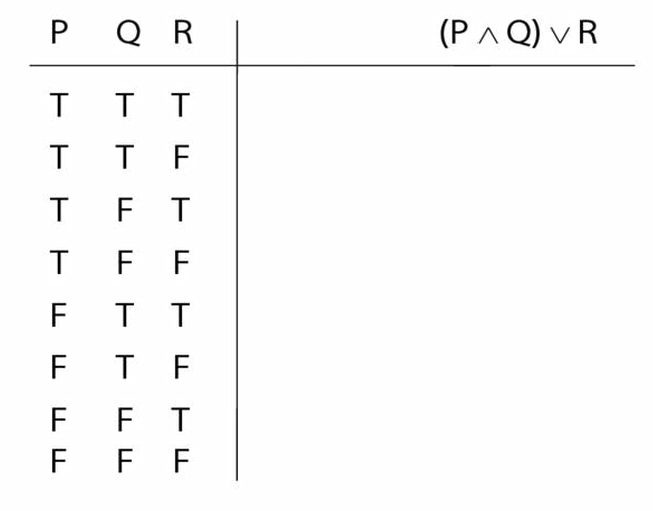
\includegraphics[scale=0.3]{img/tt_p_and_q_or_r.png}
\end{center}
\end{minipage}
 
 
 
\section{Logical Validity and Truth Tables}
 
\emph{Reading:} §4.3
 

 
\begin{minipage}{\columnwidth}
 
To establish that an argument is valid:
 
\begin{enumerate}
 
\item Create truth tables for each premise and the conclusion.
 
\item Check whether there is a row of the truth table where all premises are true and the conclusion is false.
 
\item If not, the argument is valid.
 
\end{enumerate}
 
\end{minipage}
 
 
 
\section{Tautologies and Contradictions}
 
\emph{Reading:} §4.1, §4.2
 
\begin{center}
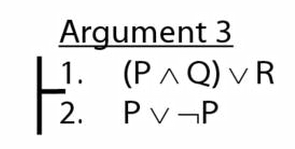
\includegraphics[scale=0.3]{img/unit_160_argument3.png}
\end{center}
\begin{center}
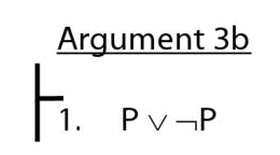
\includegraphics[scale=0.3]{img/unit_160_argument3b.png}
\end{center}
\begin{center}
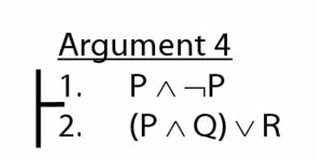
\includegraphics[scale=0.3]{img/unit_160_argument4.png}
\end{center}
P $\lor{}$ ¬P is a \emph{logical truth}
 
logical truth defined p. 568
 
P $\lor{}$ ¬P is a \emph{contradiction}
 
contradiction defined p. 564
 
\vfill
\begin{minipage}{\columnwidth}
\section{Exercises}
These exercises will be discussed in seminars the week after this lecture.
The numbers below refer to the numbered exercises in the course textbook, e.g. `1.1' refers to exercise 1.1. on page 39 of the second edition of \emph{Language, Proof and Logic}.
 
\begin{quote}
2.8, 2.10, 2.12, 2.21
 
3.1, 3.3
 
3.5, 3.7
 
3.14, 3.15
 
4.1, 4.2
 
4.12--4.16
 
\end{quote}
\end{minipage}

%--- end paste
%--------------- 
 

\end{multicols*}

\end{document}